\section{Preliminaries}
\label{sec:preliminaries}

Here we introduce some definitions, extending those in e.g.~\cite{AFSVQ21,AFSVQ23}.


\begin{definition}\label{def:plts}
    Let $\PROP$ be a countable set of propositional symbols and let $\AGT$ be a finite set of agents.  
    A \emph{Probabilistic Labeled Transition System (PLTS)}  is a tuple
    $\model=\tup{\S,\ACT,\dist(\S),\ra,\sim,\V}$ such that:
    \begin{itemize}
        \item $\S$ is a countably non-empty set of states,
        \item $\ACT$ is a countable set of action symbols,
        \item $\dist(\S)$ is the set of probability distributions over $\S$,
        \item ${\ra} \subseteq \S \times \ACT \times \dist(\S)$ is a transition relation,
        \item ${\sim}$ is a collection of relations ${\sim_i}\subseteq \DS{i}\times \DS{i}$ for each $\in\AGT$, where $\DS{i}\subseteq\ACT^*$ and every $\sim_i$ is an equivalence relation over $\DS{i}$, and 
        \item $\V: \S \ra 2^\PROP$ is a valuation function.
    \end{itemize}
    Elements of $\ACT^*$ are called \emph{plans}, and each $\sim_i$ is called the indistinguishability relation between plans for agent $i$. 
    % We write $\plan\sim_i\plan'$ whenever $(\plan,i,\plan')\in{\sim}$, and we define $\DS{i}:=\set{\plan \mid \text{ there is } \plan' \text{ s.t. } \plan\sim_i\plan'}$. 
    By $[\plan]_{\sim_i}:=\set{\plan' \in \DS{i} \mid \plan \sim_i \plan'}$ we denote $\plan$'s equivalence relation with respect to $\DS{i}$, then we define $\Unc(i) := \set{[\plan]_{\sim_i} \mid \plan\in\DS{i}}$. The set $\Unc:=\set{\Unc(i) \mid i\in\AGT}$ is called the \emph{uncertainty set} of $\model$. For simplicity sake, we sometimes denote $\model=\tup{\S,\ACT,\dist(\S),\ra,\Unc,\V}$ to refer to a PLTS, i.e., we will use its uncertainty set instead of the indistinguishability relation.
\end{definition}

Notice that, as it is defined in~\cite{AFSVQ21,AFSVQ23}, $\Unc(i)$ represents the perception agent $i$ has about the reality. In turn, the relation $\sim_i$ is not an equivalence relation over $\ACT^*$ but over $\DS{i}$, as the latter contains only the plans she considers available or suitable for her purposes, while those in $\ACT^*\setminus\DS{i}$ are not considered by $i$, even if they are suitable plans. 

\begin{definition} \label{def:executability} \raul{TBC}
    Let  $\model=\tup{\S,\ACT,\dist(\S),\ra,\Unc,\V}$ be a PLTS, let $\plan\in\ACT^*$ be a plan, and let $q\in[0,1]$ a probability, we need to define two notions:
    \begin{enumerate}
        \item We say $\plan$ is \emph{$q$-executable} at $s\in\S$ iff ...  Extend it for set of plans and set of states.
        \item For $s,t\in\S$, we write $s \reach{\plan}_q t$ iff ... Extend it for set of plans and set of states.
    \end{enumerate}
\end{definition}

\begin{center}
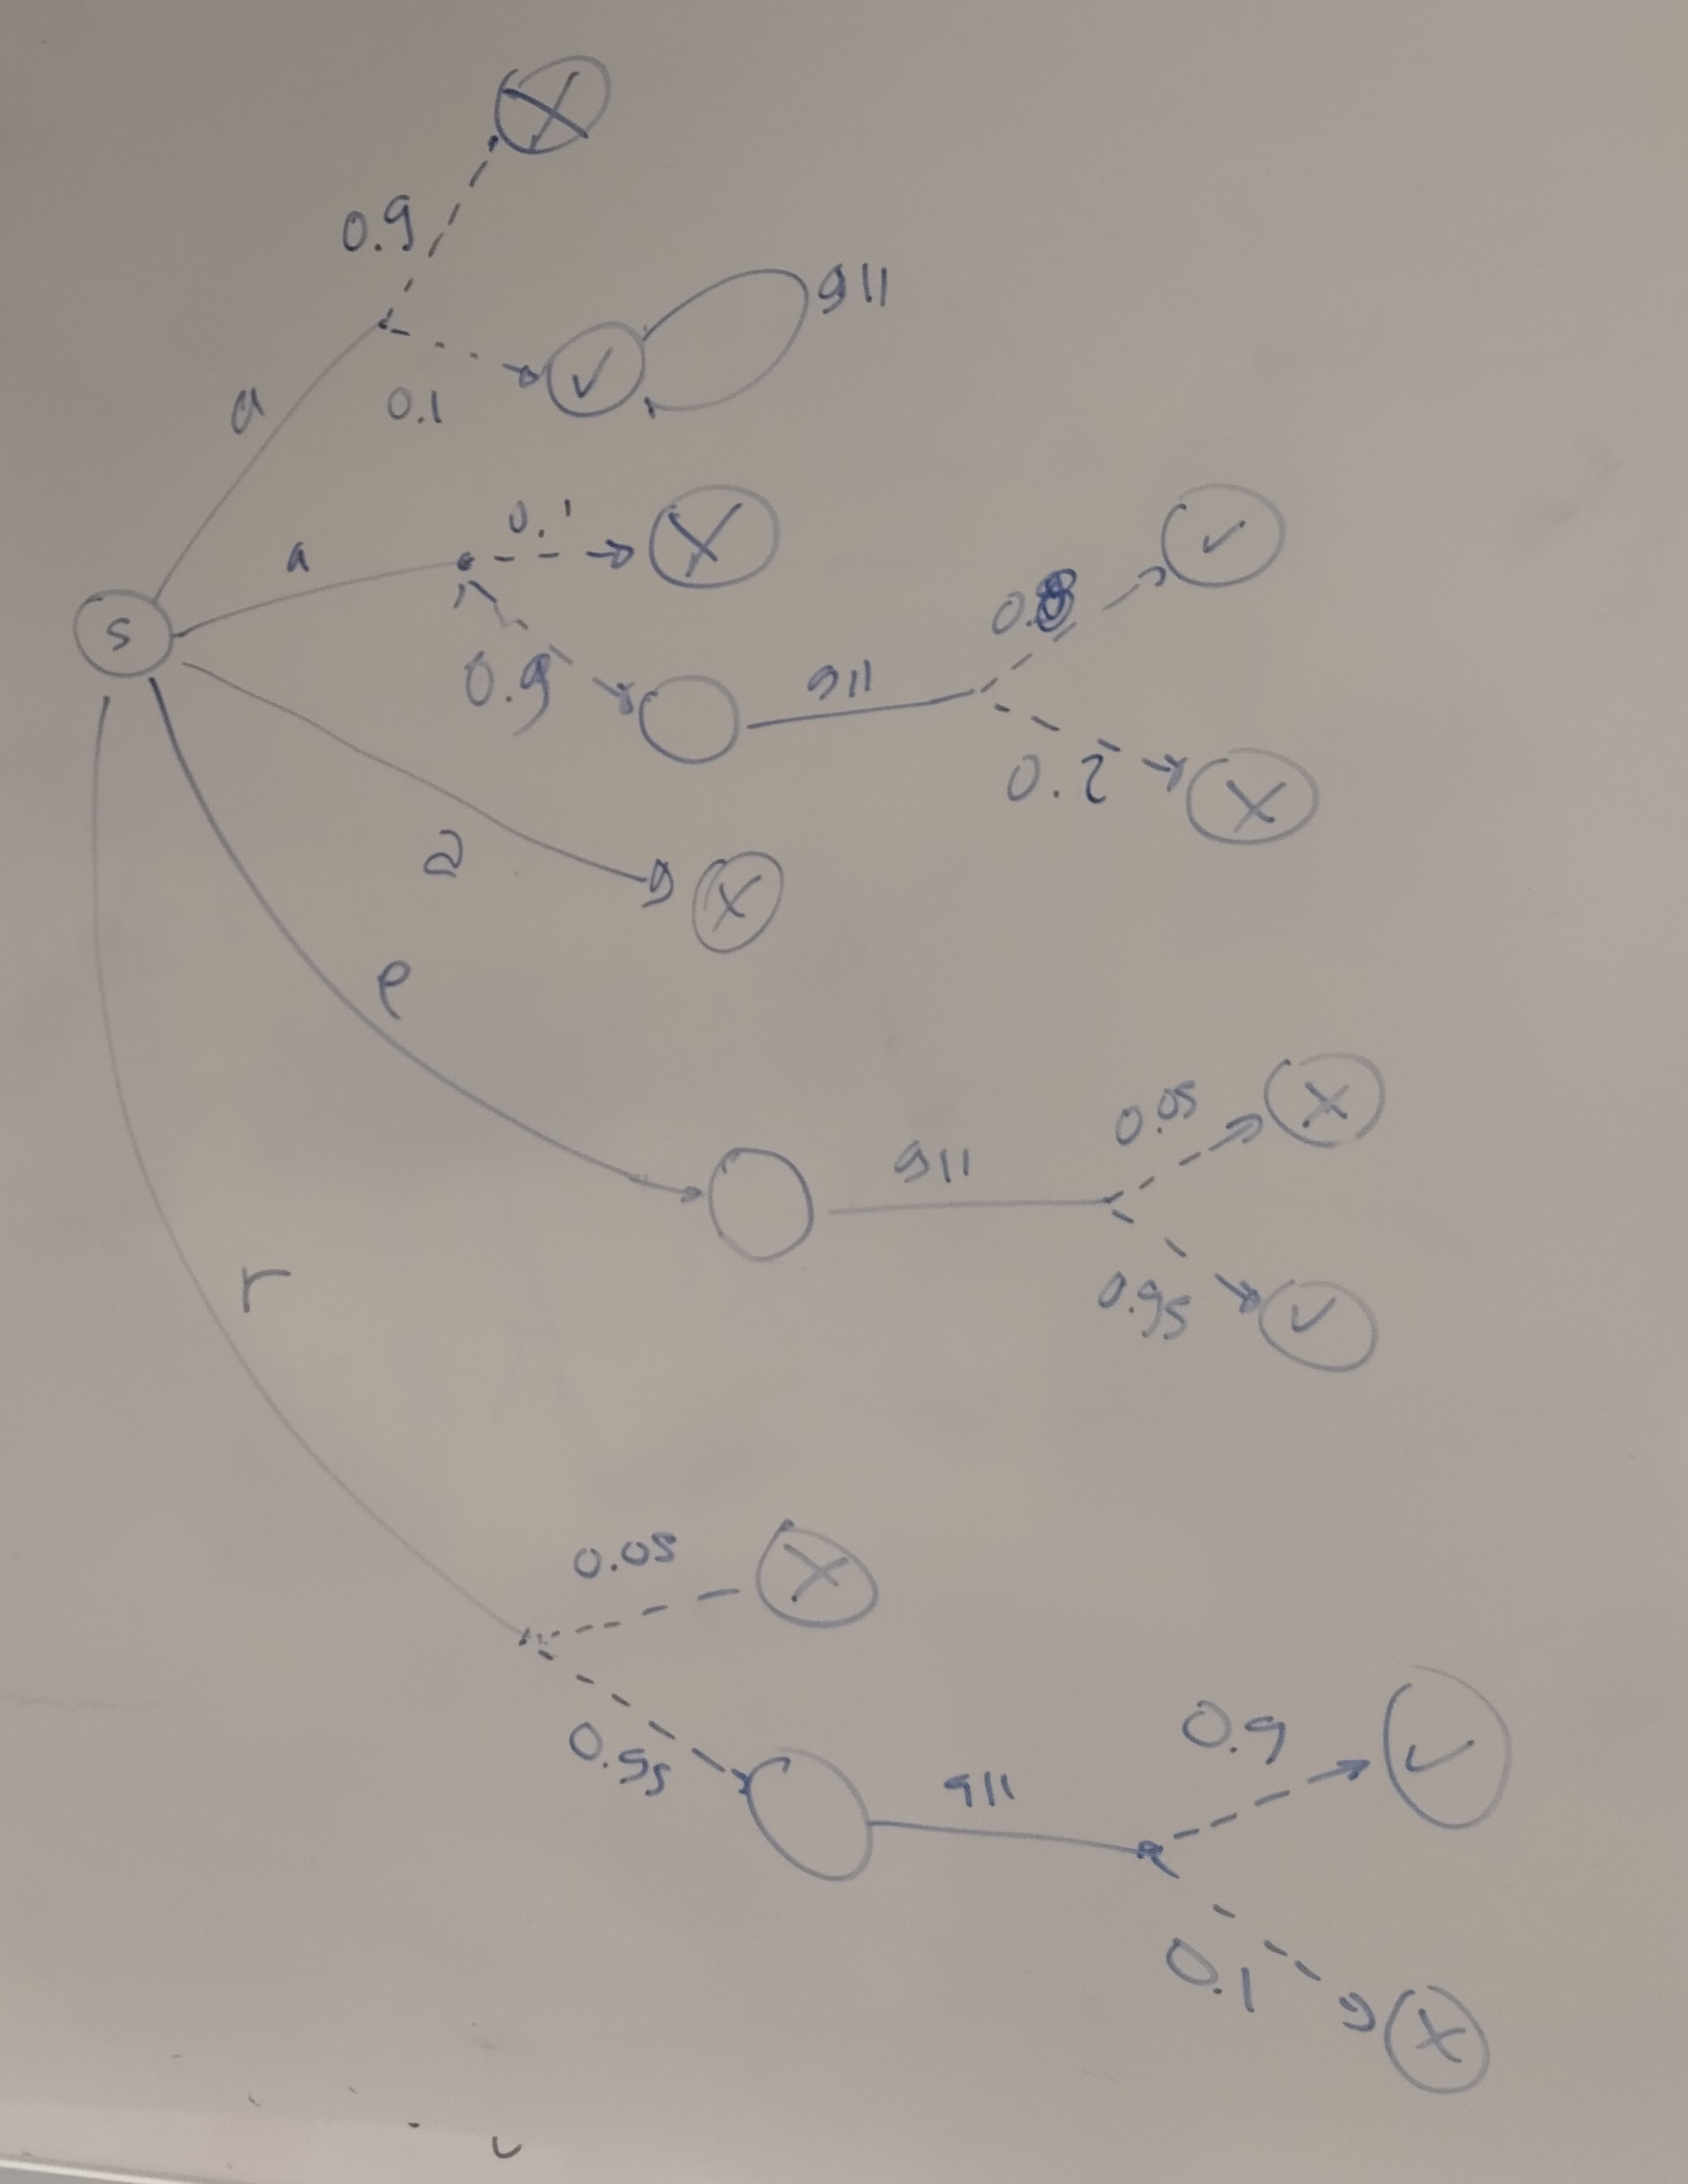
\includegraphics[scale=0.1]{PLTS.jpg}
\end{center}


In general, we will assume that PLTS are complete, as for those we can always complete the execution of a plan to a \emph{sink state}.

\begin{definition}
    \label{def:syntax}
    The set of formulas (a.k.a. the language) of $\PKh$ is defined by the following BNF:
    \[
        \varphi, \psi ::= p \mid \neg \varphi \mid \varphi \vee \psi \mid \kh_i^q(\psi,\varphi),
    \]
    where $p\in\PROP$, $i\in\AGT$ and $q\in[0,1]$. Other Boolean operators are defined as usual. Formulas of the form $\kh_i^q(\psi,\varphi)$ are read as \emph{``agent $i$ knows how to achieve $\varphi$ given $\psi$, with probability $q$''}
\end{definition}

\begin{definition} \label{def:semantics}
    Let $\model = \tup{\S,\ACT,\dist(\S),\ra,\Unc,\V}$ be a PLTS and let $s\in\S$, the satisfiability relation $\models$ for $\PKh$ is inductively defined as:
    \[
    \begin{array}{l@{\ \ \ }c@{\ \ \  }l}
    \model, s \models p & \iffdef & p \in \V(s) \\
    \model, s\models \neg\varphi & \iffdef & \model, s \not\models \varphi \\
    \model, s \models \psi\vee\varphi & \iffdef & \model, s \models \psi \mbox{ or }\model, w \models \varphi \\
    \model, s \models \kh_i^q(\psi,\varphi) & \iffdef & \text{there is } \plans \in \Unc(i) \;\text{such that:} \\
    & & \ \ \text{\rm (1)} \ \plans \text{ is $q$-executable at }  \truthset{\model}{\psi}\; \text{and} \\
    & & \ \ \text{\em (2)} \ \truthset{\model}{\psi} \reach{\plans} \truthset{\model}{\varphi}, 
    \end{array}
    \]     \raul{$q$-executable and $ \reach{\plans}_q$ to be defined}
    \noindent where: $\truthset{\model}{\chi} := \csetsc{s\in\S}{\model,w\models\chi}$. Define: $\model\models\varphi$ iff  $\truthset{\model}{\varphi}=\S$, and $\models\varphi$ iff $\model\models\varphi$, for all PLTS $\model$.
\end{definition}

The general idea in condition 1 of the clause for $\kh$ establishes that all the plans in $\plans$ have a probablity of at least $q$ of succeeding. Since all plans in $\plans$ are indistinguishability, this needs to be guaranteed no matter which plan is chosen. However, there are at least two alternatives in this definition: one considering \emph{adaptability}, meaning that there is at least one possible execution of each plan in $\plans$ for which probability $q$ is guaranteed, and considering \emph{non-adaptability} whenever we need this guarantee on each possible execution of every plan in $\plans$. Condition 2 establishes that successfull states are reached with probability of at least $q$.

\begin{remark}
    Notice that an equivalence class $\plans$ can be defined in terms of a Deterministic Finite State Automata (DFA) $\mathcal{A}_{\plans}$. This way, the operation of checking $q$-executability can be perfomed over the product $\model\times\mathcal{A}_{\plans}$. In short, $\plans$ is $q$-executable at $s$ iff for each $\plan\in\plans$, there exists one MDP in  $\model\times\mathcal{A}_{\plans}$ in which the probability of executing $\plan$ is at least $q$. This will be used while designing a model-checking algorithm (connected with algorithms from~\cite{AFSVQ21,AFSVQ23,DF23}).
\end{remark}